% Provenance (never printed): cycle 4 SVT, "La planete Terre": earthquakes,
% faults, seismic waves and their recording, magnitude and intensity, the
% link with plate boundaries; natural hazards (tsunamis) and prevention; see
% sources/book1/PROVENANCE.md. Book 1, grade 7, chapter 3.
% Vocabulary guard: P and S waves are named in prose only (they were named in
% g6.4, defined in Book 2 g11); "sediment" not before g7.4; "intensity" is
% always the earthquake's (homograph with physics: linker STOP list).
\chapter{Les séismes}\label{ch:g7:earthquakes}

Le matin du 26~décembre 2004, sous la \omterm{def:g2:water-on-earth:ocean}{mer}, au large de la pointe nord-ouest
de Sumatra, en Indonésie, les \omterm{def:g3:stones-pebbles-sand:rock}{roches} se sont rompues le long d'une
\omterm{def:g7:earthquakes:fault}{faille}~: ce fut l'un des plus grands \omterm{def:g4:volcanoes-earthquakes-first-look:earthquake}{séismes} jamais mesurés. Sur la \omterm{def:g1:landscapes-around-us:water}{côte}
voisine de Sumatra, la \omterm{def:g2:water-on-earth:ocean}{mer} s'est soulevée en vagues hautes de
\qty{51}{m}, qui ont déferlé jusqu'à \qty{5}{km} à l'intérieur des terres.
Dans les heures suivantes, les vagues ont traversé l'\omterm{def:g2:water-on-earth:ocean}{océan} Indien et
frappé les \omterm{def:g1:landscapes-around-us:water}{côtes} de quinze pays, jusqu'en Afrique. Environ 230\,000
personnes sont mortes. Il n'existait alors aucun système d'alerte dans
l'\omterm{def:g2:water-on-earth:ocean}{océan} Indien.
% ledger: usgs:largest, nws:tsunami-2004

\begin{omfigure}
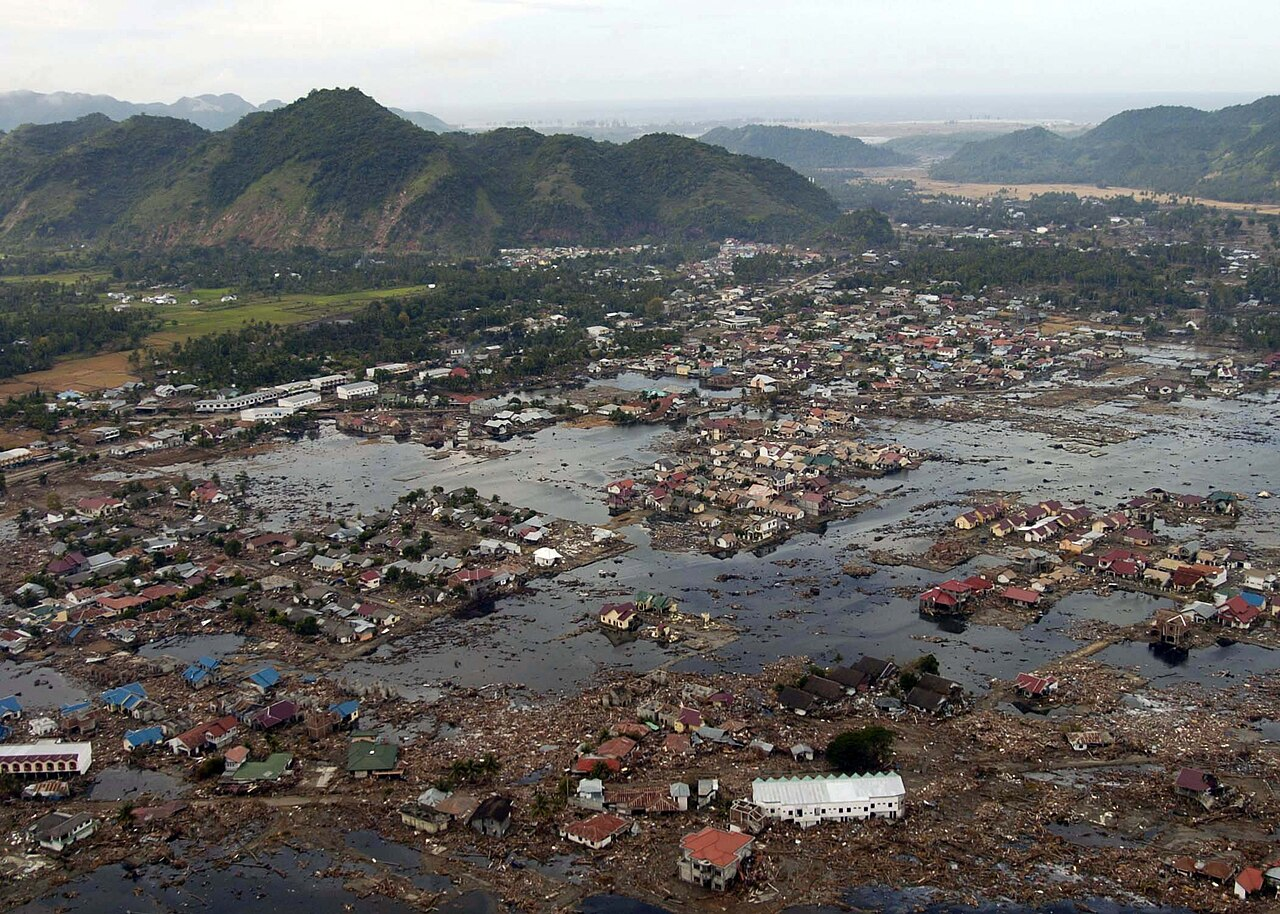
\includegraphics[width=0.78\linewidth]{images/book1/g7-tsunami-village.jpg}

{\small Un village près de la \omterm{def:g1:landscapes-around-us:water}{côte} de Sumatra, une semaine après le
\omterm{def:g7:earthquakes:tsunami}{tsunami} du 26~décembre 2004. Photographie de l'U.S. Navy, par
Philip~A. McDaniel (domaine public, via Wikimedia Commons).}
% ledger: commons:tsunami-village
\label{fig:g7:earthquakes:tsunami-village}
\end{omfigure}

Comment les \omterm{def:g3:stones-pebbles-sand:rock}{roches} se rompent-elles~? Comment les scientifiques
trouvent-ils, en quelques minutes, où un \omterm{def:g4:volcanoes-earthquakes-first-look:earthquake}{séisme} a frappé et quelle était
sa taille~? Et pourquoi la \omterm{def:g2:water-on-earth:ocean}{mer}, des heures plus tard, s'est-elle soulevée
sur des \omterm{def:g1:landscapes-around-us:water}{côtes} où personne n'avait rien senti~?

\begin{recall}
Un \emph{\omterm{def:g4:volcanoes-earthquakes-first-look:earthquake}{séisme}} est une secousse soudaine du sol, causée par des \omterm{def:g3:stones-pebbles-sand:rock}{roches}
qui se rompent et glissent, en profondeur
(\cref{ch:g4:volcanoes-earthquakes-first-look}). L'enveloppe externe de la
Terre est faite de \omterm{def:g7:plate-tectonics:plate}{plaques}, et 92~\% des grands \omterm{def:g4:volcanoes-earthquakes-first-look:earthquake}{séismes} se produisent à
moins de \qty{300}{km} d'une \omterm{def:g7:plate-tectonics:plate-boundary}{limite de plaques}
(\cref{ch:g7:plate-tectonics}). Quand un \omterm{def:g4:volcanoes-earthquakes-first-look:earthquake}{séisme} frappe, des ondes
traversent les \omterm{def:g3:stones-pebbles-sand:rock}{roches} de toute la Terre~: une sorte plus rapide (les
ondes~P) et une sorte plus lente (les ondes~S)~; en mesurant leurs temps
de parcours, les scientifiques ont découvert le \omterm{def:g6:inside-the-earth:layers}{noyau}
(\cref{ch:g6:inside-the-earth}).
\end{recall}

\section{Des roches qui se rompent}

Les \omterm{def:g7:plate-tectonics:plate}{plaques} se déplacent de quelques centimètres par an, mais leurs bords
sont rugueux~: ils restent collés l'un à l'autre pendant que le reste des
\omterm{def:g7:plate-tectonics:plate}{plaques} continue d'avancer. Les \omterm{def:g3:stones-pebbles-sand:rock}{roches} proches du bord se courbent un peu,
comme une règle que l'on pousse par les deux bouts, et accumulent de
l'énergie. Quand la poussée finit par vaincre le frottement, les \omterm{def:g3:stones-pebbles-sand:rock}{roches} se
décollent d'un coup et glissent~: ce glissement soudain, c'est le \omterm{def:g4:volcanoes-earthquakes-first-look:earthquake}{séisme}.
% ledger: usgs:eq-basics

\begin{definition}[Faille]\label{def:g7:earthquakes:fault}
Une \emph{faille}\index{faille} est une cassure dans les \omterm{def:g3:stones-pebbles-sand:rock}{roches} le long de
laquelle les deux blocs situés de part et d'autre se sont déplacés l'un par
rapport à l'autre. Pendant un \omterm{def:g4:volcanoes-earthquakes-first-look:earthquake}{séisme}, les blocs glissent brusquement le long
de la faille~; plus la faille et le glissement sont grands, plus le \omterm{def:g4:volcanoes-earthquakes-first-look:earthquake}{séisme}
est fort.
\end{definition}

Une \omterm{def:g7:plate-tectonics:plate-boundary}{limite de plaques} est faite de nombreuses \omterm{def:g7:earthquakes:fault}{failles}, et la plupart des
\omterm{def:g4:volcanoes-earthquakes-first-look:earthquake}{séismes} du monde s'y produisent. Mais il existe aussi des \omterm{def:g7:earthquakes:fault}{failles} à
l'intérieur des \omterm{def:g7:plate-tectonics:plate}{plaques}, et certaines peuvent rompre elles aussi. Quand une
grande \omterm{def:g7:earthquakes:fault}{faille} rompt près de la surface, le glissement se voit sur le
sol~: une marche dans un champ, une route coupée en deux, une clôture ou
une rangée d'arbres décalée de côté.
% ledger: usgs:eq-basics

\begin{omfigure}
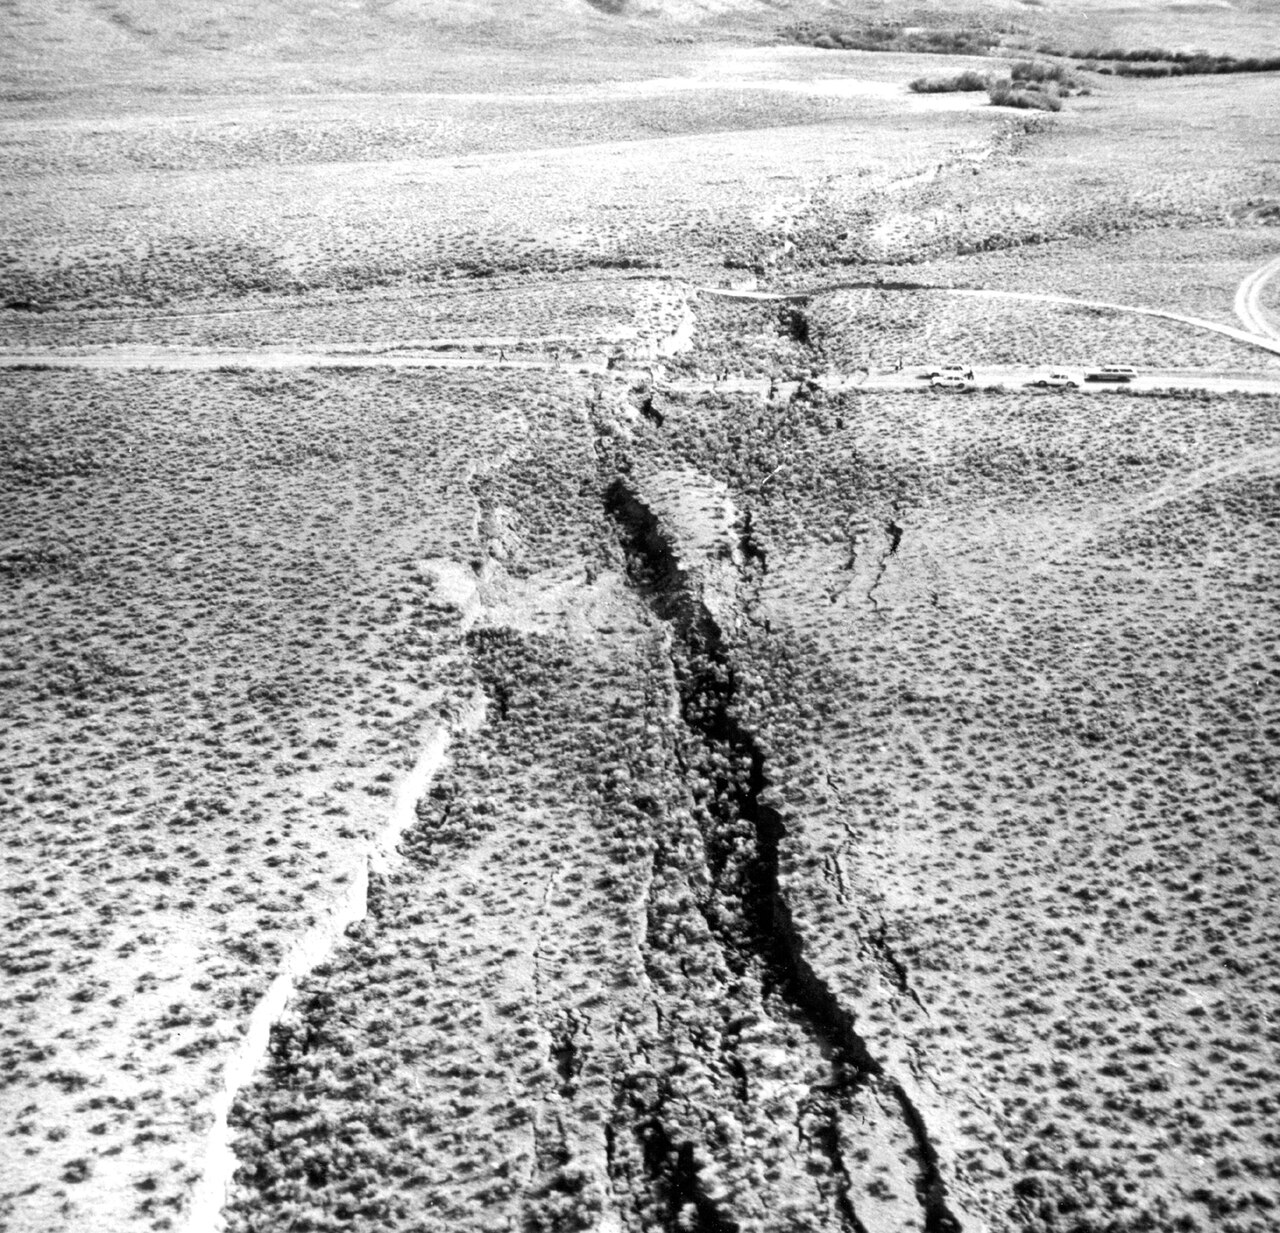
\includegraphics[width=0.62\linewidth]{images/book1/g7-borah-scarp.jpg}

{\small Les marches laissées dans le sol par le \omterm{def:g4:volcanoes-earthquakes-first-look:earthquake}{séisme} de Borah Peak, en
1983, dans l'Idaho (États-Unis), vues d'avion~: le long de la \omterm{def:g7:earthquakes:fault}{faille}, un
côté s'est abaissé par rapport à l'autre, et la marche traverse la route en
haut de l'image. Photographie~: R.~E. Wallace, U.S. Geological Survey
(domaine public, via Wikimedia Commons).}
% ledger: commons:borah-scarp
\label{fig:g7:earthquakes:borah}
\end{omfigure}

\begin{definition}[Foyer et épicentre]\label{def:g7:earthquakes:focus}
Le \emph{foyer}\index{foyer} d'un \omterm{def:g4:volcanoes-earthquakes-first-look:earthquake}{séisme} est l'endroit, en profondeur, sur
la \omterm{def:g7:earthquakes:fault}{faille}, où le glissement commence. L'\emph{épicentre}\index{epicentre@épicentre}
est le point de la surface de la Terre situé juste au-dessus du foyer.
\end{definition}

Le \omterm{def:g7:earthquakes:focus}{foyer} se trouve souvent à quelques kilomètres ou à quelques dizaines de
kilomètres de profondeur. Sur les 7\,031 \omterm{def:g4:volcanoes-earthquakes-first-look:earthquake}{séismes} de \omterm{def:g7:earthquakes:magnitude}{magnitude}~6 ou plus
enregistrés entre 1976 et 2025, 5\,561 --- soit 79~\% --- avaient leur
\omterm{def:g7:earthquakes:focus}{foyer} à moins de \qty{70}{km} de profondeur. Mais 483 ont commencé à plus
de \qty{300}{km} de profondeur, et le plus profond à \qty{688}{km}~: ces
\omterm{def:g4:volcanoes-earthquakes-first-look:earthquake}{séismes} profonds se produisent là où une \omterm{def:g7:plate-tectonics:plate}{plaque} s'enfonce sous une autre,
à l'intérieur de la \omterm{def:g7:plate-tectonics:plate}{plaque} qui s'enfonce.
% ledger: data:usgs-comcat (figdata/grade-7/quake_counts.py, part depth)

Un grand \omterm{def:g4:volcanoes-earthquakes-first-look:earthquake}{séisme} arrive rarement seul. Il est souvent suivi, au même
endroit, de \omterm{def:g4:volcanoes-earthquakes-first-look:earthquake}{séismes} plus petits, les \emph{répliques}, pendant des
semaines, des mois, et même des années. Parfois, de plus petits \omterm{def:g4:volcanoes-earthquakes-first-look:earthquake}{séismes} le
précèdent, mais personne ne peut savoir que c'étaient des avertissements
avant que le grand \omterm{def:g4:volcanoes-earthquakes-first-look:earthquake}{séisme} ne se soit produit~: les scientifiques ne savent
pas prévoir les \omterm{def:g4:volcanoes-earthquakes-first-look:earthquake}{séismes}. Ils peuvent seulement dire quelles \omterm{def:g7:earthquakes:fault}{failles}
rompront de nouveau un jour, et aider les gens à se préparer.
% ledger: usgs:eq-basics, usgs:seismograph

\begin{omfigure}
\begin{tikzpicture}[font=\small, x=1cm, y=1cm]
  % a block of crust seen in perspective: front face and top face
  \def\dx{2.2}\def\dy{1.3}
  % top surface: two blocks separated by the fault trace
  \fill[green!12] (0,0) -- (4.6,0) -- (4.6+\dx,\dy) -- (\dx,\dy) -- cycle;
  \fill[green!18] (4.6,0) -- (9,0) -- (9+\dx,\dy) -- (4.6+\dx,\dy) -- cycle;
  % front face
  \fill[brown!30] (0,0) -- (4.6,0) -- (3.4,-4) -- (0,-4) -- cycle;
  \fill[brown!40] (4.6,0) -- (9,0) -- (9,-4) -- (3.4,-4) -- cycle;
  % right face
  \fill[brown!22] (9,0) -- (9+\dx,\dy) -- (9+\dx,\dy-4) -- (9,-4) -- cycle;
  % fault plane on the front face and trace on top
  \draw[very thick, red!70!black] (4.6,0) -- (3.4,-4);
  \draw[very thick, red!70!black] (4.6,0) -- (4.6+\dx,\dy);
  % slip arrows
  \draw[-{Stealth[length=2.5mm]}, thick] (2.6,-0.35) -- (1.6,-0.35);
  \draw[-{Stealth[length=2.5mm]}, thick] (6.4,-0.35) -- (7.4,-0.35);
  \node[font=\footnotesize, anchor=south] at (2.1,-0.3) {bloc 1};
  \node[font=\footnotesize, anchor=south] at (6.9,-0.3) {bloc 2};
  % focus and waves
  \coordinate (F) at (3.95,-2.4);
  \foreach \r in {0.5,1.0,1.5,2.0}
    \draw[blue!60, dashed] (F) circle (\r);
  \fill[red!80!black] (F) circle (0.13);
  % epicentre: on the surface, straight above the focus (front edge of the top face)
  \coordinate (E) at (3.95,0);
  \draw[black!60, densely dotted, thick] (F) -- (E);
  \node[star, star points=5, star point ratio=2.4, fill=orange, draw=black, inner sep=1.4pt] at (E) {};
  % labels
  \node[anchor=west] at (9.5,-2.3) {foyer};
  \draw[black!60] (9.45,-2.3) -- (4.1,-2.4);
  \node[anchor=south west] at (4.9,1.9) {épicentre};
  \draw[black!60] (4.95,1.95) -- (4.05,0.12);
  \node[anchor=south, red!70!black] at (6.8,1.3) {faille};
  \node[anchor=east, blue!60!black, align=right] at (-0.15,-2.6) {des ondes partent\\dans toutes les directions};
  \draw[blue!60, -{Stealth}] (-0.1,-2.6) -- (1.9,-2.5);
\end{tikzpicture}

{\small Une \omterm{def:g7:earthquakes:fault}{faille}, le \omterm{def:g7:earthquakes:focus}{foyer} et l'\omterm{def:g7:earthquakes:focus}{épicentre} (un dessin, pas à l'échelle).
Les deux blocs glissent l'un contre l'autre le long de la \omterm{def:g7:earthquakes:fault}{faille} (en
rouge)~; le glissement commence au \omterm{def:g7:earthquakes:focus}{foyer}, et des ondes en partent dans
toutes les directions, comme des ronds dans l'eau. L'\omterm{def:g7:earthquakes:focus}{épicentre} (étoile)
est à la surface, juste au-dessus du \omterm{def:g7:earthquakes:focus}{foyer}.}
% ledger: usgs:eq-basics
\label{fig:g7:earthquakes:fault}
\end{omfigure}


\section{Enregistrer un séisme}

\begin{definition}[Sismomètre et sismogramme]\label{def:g7:earthquakes:seismometer}
Un \emph{sismomètre}\index{sismometre@sismomètre} est un instrument qui
enregistre les secousses du sol. Son enregistrement, une ligne ondulée
tracée en fonction du temps, est un
\emph{sismogramme}\index{sismogramme}.
\end{definition}

Le principe d'un \omterm{def:g7:earthquakes:seismometer}{sismomètre} est simple. Un bâti est solidement fixé au
sol~; une lourde masse y est suspendue par un ressort. Quand le sol
tremble, le bâti tremble avec lui, mais la lourde masse, tenue seulement
par son ressort, reste presque immobile. L'instrument enregistre le
mouvement du bâti par rapport à la masse immobile~: c'est le mouvement du
sol. Sur le dessin ci-dessous, un stylet fixé à la masse le trace sur un
papier enroulé autour d'un tambour qui tourne.
% ledger: usgs:seismograph

\begin{omfigure}
\begin{tikzpicture}[font=\small, x=1cm, y=1cm]
  \begin{scope}
    % ground
    \fill[brown!30] (-0.6,-0.6) rectangle (5.0,0);
    \draw[decorate, decoration={snake, amplitude=1.2pt, segment length=6pt}, brown!70!black, thick]
      (-0.6,0) -- (5.0,0);
    % frame
    \fill[black!55] (0,0) rectangle (0.25,3.2);
    \fill[black!55] (0,3.0) rectangle (2.4,3.25);
    % spring and weight
    \draw[decorate, decoration={coil, aspect=0.5, segment length=3pt, amplitude=4pt}, thick]
      (2.1,3.0) -- (2.1,2.1);
    \fill[black!80] (1.7,1.45) rectangle (2.5,2.1);
    \node[white, font=\scriptsize] at (2.1,1.78) {masse};
    % pen arm and drum
    \draw[thick] (2.5,1.75) -- (3.45,1.75);
    \fill (3.45,1.75) circle (0.05);
    \draw[thick, fill=white] (3.95,1.75) circle (0.5);
    \draw[thick] (3.95,1.25) -- (3.95,0);
    \draw[-{Stealth}, black!60] (4.55,2.2) arc (40:-40:0.7);
    % labels
    \node[anchor=east, align=right, font=\footnotesize] at (-0.1,2.3) {bâti fixé\\au sol};
    \node[anchor=west, font=\footnotesize] at (2.6,2.65) {ressort};
    \draw[black!60] (2.55,2.65) -- (2.25,2.6);
    \node[anchor=north, align=center, font=\footnotesize] at (2.1,1.35) {masse lourde~:\\reste immobile};
    \node[anchor=west, align=left, font=\footnotesize] at (4.7,1.05) {tambour qui tourne,\\avec du papier};
    \node[anchor=north, font=\footnotesize] at (2.2,-0.65) {le sol tremble};
  \end{scope}
  \begin{scope}[xshift=7.2cm, yshift=0.4cm]
    \begin{axis}[width=7.6cm, height=4.2cm, xmin=0, xmax=60, ymin=-1.1, ymax=1.1,
        axis x line=bottom, axis y line=none, xlabel={temps (secondes)},
        tick label style={font=\scriptsize}, label style={font=\footnotesize}, clip=false]
      \addplot[black, line width=0.4pt] table[x=t, y=v] {figdata/out/grade-7-epicentre-m-trace.dat};
      \draw[blue!70!black, -{Stealth[length=2mm]}] (axis cs:10,1.45) -- (axis cs:10,0.45);
      \node[blue!70!black, font=\scriptsize, anchor=south east] at (axis cs:10.5,1.45) {arrivée des ondes rapides};
      \draw[red!70!black, -{Stealth[length=2mm]}] (axis cs:20,1.45) -- (axis cs:20,1.05);
      \node[red!70!black, font=\scriptsize, anchor=south west] at (axis cs:19.5,1.45) {arrivée des ondes lentes};
      \draw[{Stealth[length=2mm]}-{Stealth[length=2mm]}] (axis cs:10,-0.75) -- (axis cs:20,-0.75);
      \node[font=\scriptsize, anchor=east] at (axis cs:9,-0.75) {décalage~: 10 s};
    \end{axis}
  \end{scope}
\end{tikzpicture}

{\small À gauche~: le principe d'un \omterm{def:g7:earthquakes:seismometer}{sismomètre} (un dessin). À droite~: un
\omterm{def:g7:earthquakes:seismometer}{sismogramme} tracé pour ce livre (pas un véritable enregistrement)~: la
ligne est calme, puis arrivent les ondes les plus rapides, puis, dix
secondes plus tard, les plus lentes, plus grandes.}
% ledger: usgs:seismograph (trace drawn by figdata/grade-7/epicentre.py, part m-trace)
\label{fig:g7:earthquakes:seismometer}
\end{omfigure}

\subsection*{À quelle distance était le séisme~?}

Un \omterm{def:g7:earthquakes:seismometer}{sismogramme} en dit plus que «~le sol a tremblé~». Les ondes les plus
rapides arrivent toujours les premières, et les plus lentes après. Près du
\omterm{def:g7:earthquakes:focus}{foyer}, elles arrivent presque ensemble~; loin du \omterm{def:g7:earthquakes:focus}{foyer}, les ondes lentes
prennent de plus en plus de retard, de même que, pendant un orage, le
tonnerre suit l'éclair avec d'autant plus de retard que l'orage est loin.
Le décalage entre les deux arrivées donne donc la distance du \omterm{def:g4:volcanoes-earthquakes-first-look:earthquake}{séisme}.
% ledger: usgs:seismograph

Combien de kilomètres pour chaque seconde de décalage~? Cela dépend des
vitesses des deux ondes dans les \omterm{def:g3:stones-pebbles-sand:rock}{roches} qu'elles traversent. Avec les
vitesses du modèle de référence de la Terre (\cref{ch:g6:inside-the-earth}),
chaque seconde de décalage correspond à environ \qty{7}{km} dans la \omterm{def:g6:inside-the-earth:layers}{croûte}
supérieure et \qty{9}{km} dans la \omterm{def:g6:inside-the-earth:layers}{croûte} inférieure. Dans les exercices de
ce chapitre, nous utilisons la valeur ronde de \qty{8}{km} par seconde.
% ledger: data:prem (computed in figdata/grade-7/epicentre.py, part rule)

\begin{method}[Trouver l'épicentre avec trois stations]\label{met:g7:earthquakes:three-circles}
\begin{enumerate}
  \item Sur le \omterm{def:g7:earthquakes:seismometer}{sismogramme} de chaque station, lis le décalage entre
        l'arrivée des ondes rapides et l'arrivée des ondes lentes.
  \item Transforme chaque décalage en distance (ici~: $8 \times$ le
        décalage en secondes, en kilomètres).
  \item Sur une \omterm{def:g2:drawing-to-map:map}{carte}, trace autour de chaque station un cercle dont le
        rayon est sa distance. L'\omterm{def:g7:earthquakes:focus}{épicentre} se trouve quelque part sur
        chaque cercle.
  \item Avec deux cercles, il y a en général deux points possibles~; le
        troisième cercle ne passe que par l'un d'eux~: c'est l'\omterm{def:g7:earthquakes:focus}{épicentre}.
\end{enumerate}
\end{method}

\begin{example}[Trois cercles]\label{ex:g7:earthquakes:three-circles}
Trois stations enregistrent le même \omterm{def:g4:volcanoes-earthquakes-first-look:earthquake}{séisme}. Les décalages sont de
\qty{10}{s} à la station~M1, \qty{11.25}{s} à M2 et \qty{9.75}{s} à M3.
Les distances sont $8 \times 10 = \qty{80}{km}$, $8 \times 11.25 = \qty{90}{km}$ et
$8 \times 9.75 = \qty{78}{km}$. Les trois cercles, tracés ci-dessous, se
coupent en un seul point~: l'\omterm{def:g7:earthquakes:focus}{épicentre}.
% ledger: usgs:seismograph (figdata/grade-7/epicentre.py, parts m-stations and m-circles)
\end{example}

\begin{omfigure}
\begin{tikzpicture}
  \begin{axis}[axis equal image, width=8.2cm, xmin=-150, xmax=170, ymin=-160, ymax=160,
      xtick={-120,-80,...,160}, ytick={-120,-80,...,120}, grid=both, grid style={black!12},
      tick label style={font=\scriptsize}, xlabel={km}, ylabel={km}, label style={font=\footnotesize}]
    \addplot[blue!60!black, line width=0.6pt] table[x=x, y=y] {figdata/out/grade-7-epicentre-m-circles.dat};
    \addplot[only marks, mark=triangle*, mark size=3pt, black,
        nodes near coords, point meta=explicit symbolic,
        nodes near coords style={font=\scriptsize, anchor=north, yshift=-2pt}]
      table[x=x, y=y, meta=name] {figdata/out/grade-7-epicentre-m-stations.dat};
    \node[star, star points=5, star point ratio=2.4, fill=orange, draw=black, inner sep=1.6pt] at (axis cs:0,0) {};
    \draw[black!60] (axis cs:-4,-4) -- (axis cs:-60,-75);
    \node[font=\scriptsize, anchor=north east, inner sep=1pt] at (axis cs:-60,-75) {épicentre};
  \end{axis}
\end{tikzpicture}

{\small Chaque cercle est centré sur une station (triangle), avec un rayon
égal à la distance entre cette station et le \omterm{def:g4:volcanoes-earthquakes-first-look:earthquake}{séisme}. Les trois cercles ne
se coupent qu'en un point, l'\omterm{def:g7:earthquakes:focus}{épicentre} (étoile).}
% ledger: usgs:seismograph (figdata/grade-7/epicentre.py, parts m-stations and m-circles)
\label{fig:g7:earthquakes:three-circles}
\end{omfigure}

\begin{omfigure}
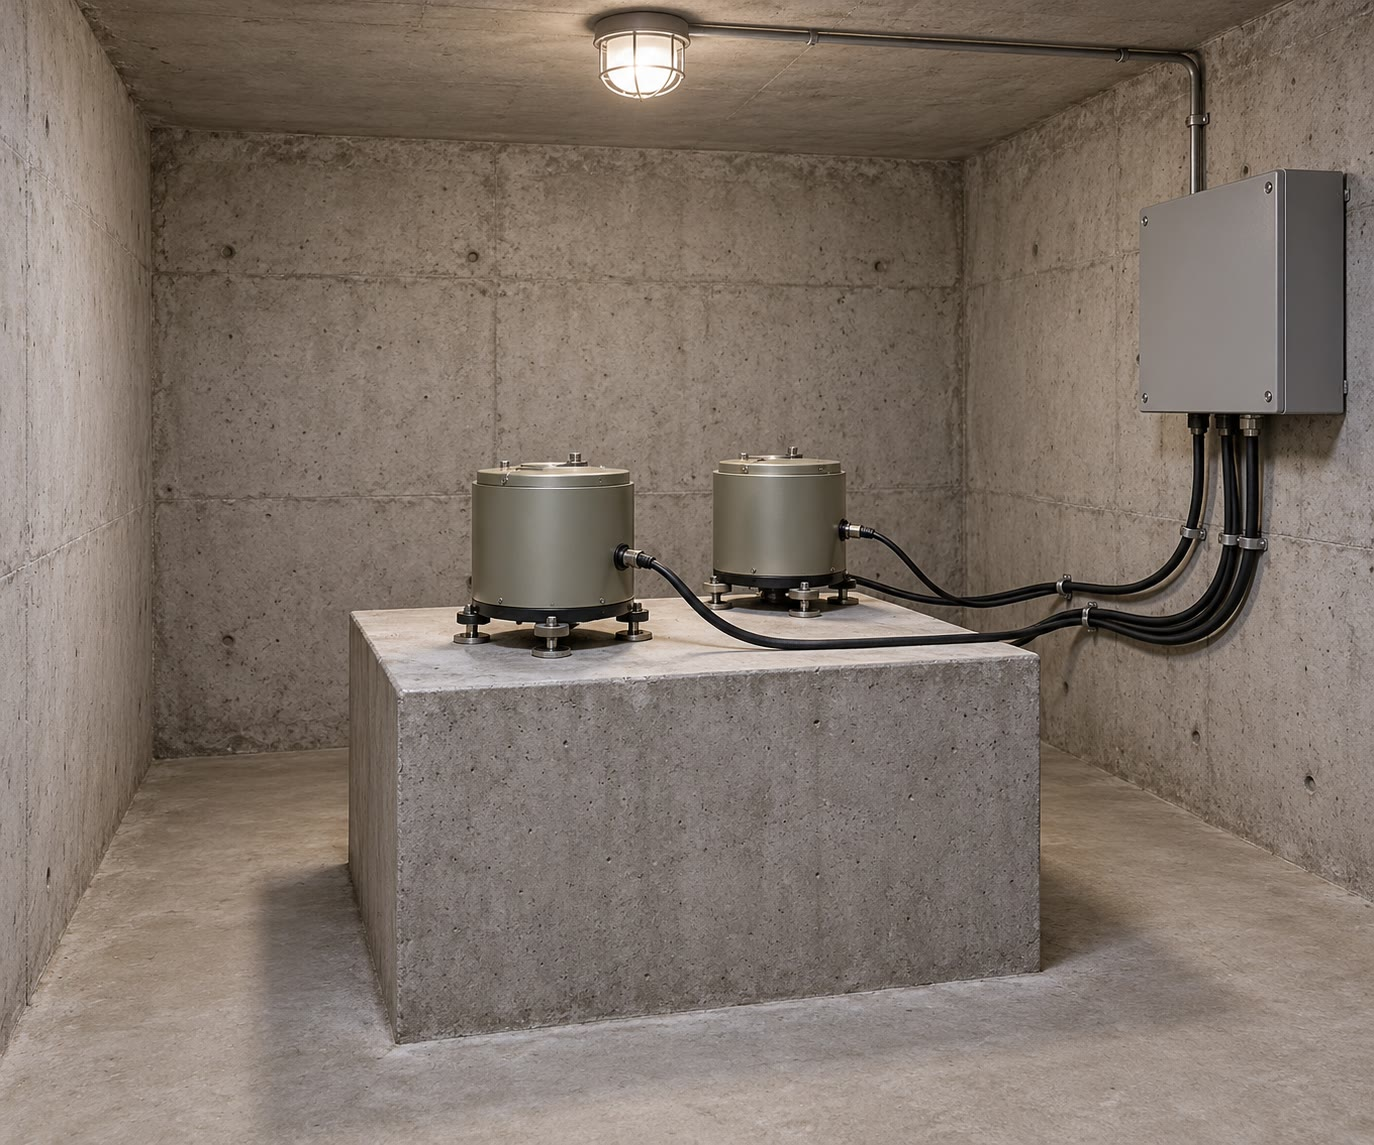
\includegraphics[width=0.58\linewidth]{images/book1/ai/g7-seismometer-vault.jpg}

{\small Des \omterm{def:g7:earthquakes:seismometer}{sismomètres} dans une salle souterraine silencieuse, posés sur
un pilier de béton qui repose sur la \omterm{def:g3:stones-pebbles-sand:rock}{roche}, loin des routes et des machines
(illustration générée par IA d'une scène générique).}
\label{fig:g7:earthquakes:vault}
\end{omfigure}

\section{Quelle taille~? Magnitude et intensité}

Deux nombres différents décrivent un \omterm{def:g4:volcanoes-earthquakes-first-look:earthquake}{séisme}, et on les confond souvent.

\begin{definition}[Magnitude]\label{def:g7:earthquakes:magnitude}
La \emph{magnitude}\index{magnitude} d'un \omterm{def:g4:volcanoes-earthquakes-first-look:earthquake}{séisme} mesure sa taille~:
l'énergie libérée au \omterm{def:g7:earthquakes:focus}{foyer}. On la calcule à partir des \omterm{def:g7:earthquakes:seismometer}{sismogrammes}.
Chaque \omterm{def:g4:volcanoes-earthquakes-first-look:earthquake}{séisme} a une seule magnitude, écrite avec une décimale, comme 6.3
ou 9.1.
\end{definition}

\begin{definition}[Intensité]\label{def:g7:earthquakes:intensity}
L'\emph{intensité}\index{intensite@intensité} d'un \omterm{def:g4:volcanoes-earthquakes-first-look:earthquake}{séisme} en un lieu décrit
la force avec laquelle le sol y a tremblé, d'après ce que les gens ont
ressenti et les dégâts qu'ils ont vus. On l'écrit en chiffres romains, de
I (non ressenti) à XII (destruction totale). Un \omterm{def:g4:volcanoes-earthquakes-first-look:earthquake}{séisme} a de nombreuses
intensités~: une différente en chaque lieu.
\end{definition}

L'échelle des \omterm{def:g7:earthquakes:magnitude}{magnitudes} monte vite. Chaque pas de 1 en \omterm{def:g7:earthquakes:magnitude}{magnitude}
correspond à des ondes environ 10~fois plus grandes sur le \omterm{def:g7:earthquakes:seismometer}{sismogramme} et
à environ 32~fois plus d'énergie libérée. Un \omterm{def:g4:volcanoes-earthquakes-first-look:earthquake}{séisme} de \omterm{def:g7:earthquakes:magnitude}{magnitude}~8 libère
environ $32 \times 32 \approx 1000$ fois plus d'énergie qu'un \omterm{def:g4:volcanoes-earthquakes-first-look:earthquake}{séisme} de
\omterm{def:g7:earthquakes:magnitude}{magnitude}~6.
% ledger: usgs:mag-energy

\begin{method}[Comparer deux magnitudes]\label{met:g7:earthquakes:magnitudes}
Pour comparer l'énergie de deux \omterm{def:g4:volcanoes-earthquakes-first-look:earthquake}{séismes}, compte les pas entiers entre
leurs \omterm{def:g7:earthquakes:magnitude}{magnitudes}, et multiplie par 32 une fois par pas~: 1~pas, 32~fois~;
2~pas, environ 1000~fois~; 3~pas, environ 32\,000~fois.
\end{method}

\begin{example}[Magnitude 9 et magnitude 7]\label{ex:g7:earthquakes:nine-seven}
Le \omterm{def:g4:volcanoes-earthquakes-first-look:earthquake}{séisme} de 2004 au large de Sumatra avait une \omterm{def:g7:earthquakes:magnitude}{magnitude} de 9.1. Un
\omterm{def:g4:volcanoes-earthquakes-first-look:earthquake}{séisme} de \omterm{def:g7:earthquakes:magnitude}{magnitude}~7.1 est plus petit de deux pas~: il a libéré environ
$32 \times 32 = 1024$, donc environ 1000~fois, moins d'énergie.
% ledger: usgs:largest, usgs:mag-energy
\end{example}

Les plus grands \omterm{def:g4:volcanoes-earthquakes-first-look:earthquake}{séismes} jamais mesurés se sont tous produits là où une
\omterm{def:g7:plate-tectonics:plate}{plaque} s'enfonce sous une autre~: \omterm{def:g7:earthquakes:magnitude}{magnitude}~9.5 au Chili le 22~mai 1960,
9.2 en Alaska en 1964, 9.1 au large de Sumatra en 2004 et 9.1 au large du
Japon le 11~mars 2011. Les grands \omterm{def:g4:volcanoes-earthquakes-first-look:earthquake}{séismes} sont rares, et d'autant plus
rares qu'ils sont grands, comme le montre le graphique~: à chaque pas de
\omterm{def:g7:earthquakes:magnitude}{magnitude} en plus, environ dix fois moins.
% ledger: usgs:largest, data:usgs-comcat

\begin{omfigure}
\begin{tikzpicture}
  \begin{axis}[ybar, width=0.72\linewidth, height=5.4cm, bar width=22pt,
      ymode=log, log origin y=infty, ymin=0.01, ymax=600,
      xtick=data, xticklabels={6 à 6.9, 7 à 7.9, 8 à 8.9, 9 ou plus},
      xlabel={magnitude}, ylabel={séismes par an},
      ytick={0.01,0.1,1,10,100}, yticklabels={0.01,0.1,1,10,100},
      tick label style={font=\scriptsize}, label style={font=\small},
      nodes near coords, point meta=explicit symbolic,
      nodes near coords style={font=\scriptsize}, enlarge x limits=0.18,
      axis x line*=bottom, axis y line*=left]
    \addplot[fill=omThm!45, draw=omThm!80!black] table[x=cls, y=per_year, meta=per_year] {figdata/out/grade-7-quake_counts.dat};
  \end{axis}
\end{tikzpicture}

{\small Nombre de \omterm{def:g4:volcanoes-earthquakes-first-look:earthquake}{séismes} par an, en moyenne sur 1976--2025, selon la
\omterm{def:g7:earthquakes:magnitude}{magnitude}. L'échelle verticale est spéciale~: chaque ligne vaut dix fois
celle du dessous. Données~: catalogue des \omterm{def:g4:volcanoes-earthquakes-first-look:earthquake}{séismes} de l'U.S. Geological
Survey (7\,031 \omterm{def:g4:volcanoes-earthquakes-first-look:earthquake}{séismes} de \omterm{def:g7:earthquakes:magnitude}{magnitude}~6 ou plus).}
% ledger: data:usgs-comcat (figdata/grade-7/quake_counts.py, main table)
\label{fig:g7:earthquakes:counts}
\end{omfigure}

L'\omterm{def:g7:earthquakes:intensity}{échelle d'intensité} n'a pas de formule~: c'est une liste de ce qui se
passe. Le tableau la donne en abrégé.
% ledger: usgs:mmi, usgs:mmi-page

\begin{center}
\small
\begin{tabular}{|c|p{0.8\linewidth}|}
\hline
\textbf{\omterm{def:g7:earthquakes:intensity}{intensité}} & \textbf{ce que l'on ressent et ce que l'on voit} \\
\hline
I & non ressenti, sauf par de très rares personnes \\
II & ressenti seulement par quelques personnes au repos, surtout dans les étages~; les objets suspendus peuvent se balancer \\
III & ressenti à l'intérieur~; on dirait le passage d'un camion \\
IV & ressenti à l'intérieur par beaucoup~; la vaisselle, les fenêtres et les portes vibrent \\
V & ressenti par presque tout le monde, beaucoup sont réveillés~; un peu de vaisselle et quelques fenêtres cassées \\
VI & ressenti par tous, beaucoup ont peur~; quelques meubles lourds déplacés~; légers dégâts \\
VII & peu de dégâts dans les bâtiments bien construits, beaucoup dans les bâtiments mal construits~; quelques cheminées cassées \\
VIII & beaucoup de dégâts dans les bâtiments ordinaires, certains s'effondrent en partie~; des cheminées et des murs tombent \\
IX & grands dégâts même dans les bâtiments solides~; des bâtiments déplacés de leurs fondations \\
X & la plupart des bâtiments détruits avec leurs fondations~; rails tordus \\
XI & peu de bâtiments restent debout~; ponts détruits \\
XII & destruction totale~; des objets projetés en l'air \\
\hline
\end{tabular}
\end{center}
% ledger: usgs:mmi

L'\omterm{def:g7:earthquakes:intensity}{intensité} est en général la plus forte près de l'\omterm{def:g7:earthquakes:focus}{épicentre}, et elle
diminue avec la distance. Mais elle dépend aussi du sol~: la \omterm{def:g3:stones-pebbles-sand:rock}{roche} dure est
celle qui tremble le moins, la \omterm{def:g3:stones-pebbles-sand:sand}{boue} molle celle qui tremble le plus. Une
ville bâtie sur un sol mou peut être secouée plus fort qu'une autre ville,
plus proche de l'\omterm{def:g7:earthquakes:focus}{épicentre} mais bâtie sur la \omterm{def:g3:stones-pebbles-sand:rock}{roche}.
% ledger: usgs:mag-energy

\begin{omfigure}
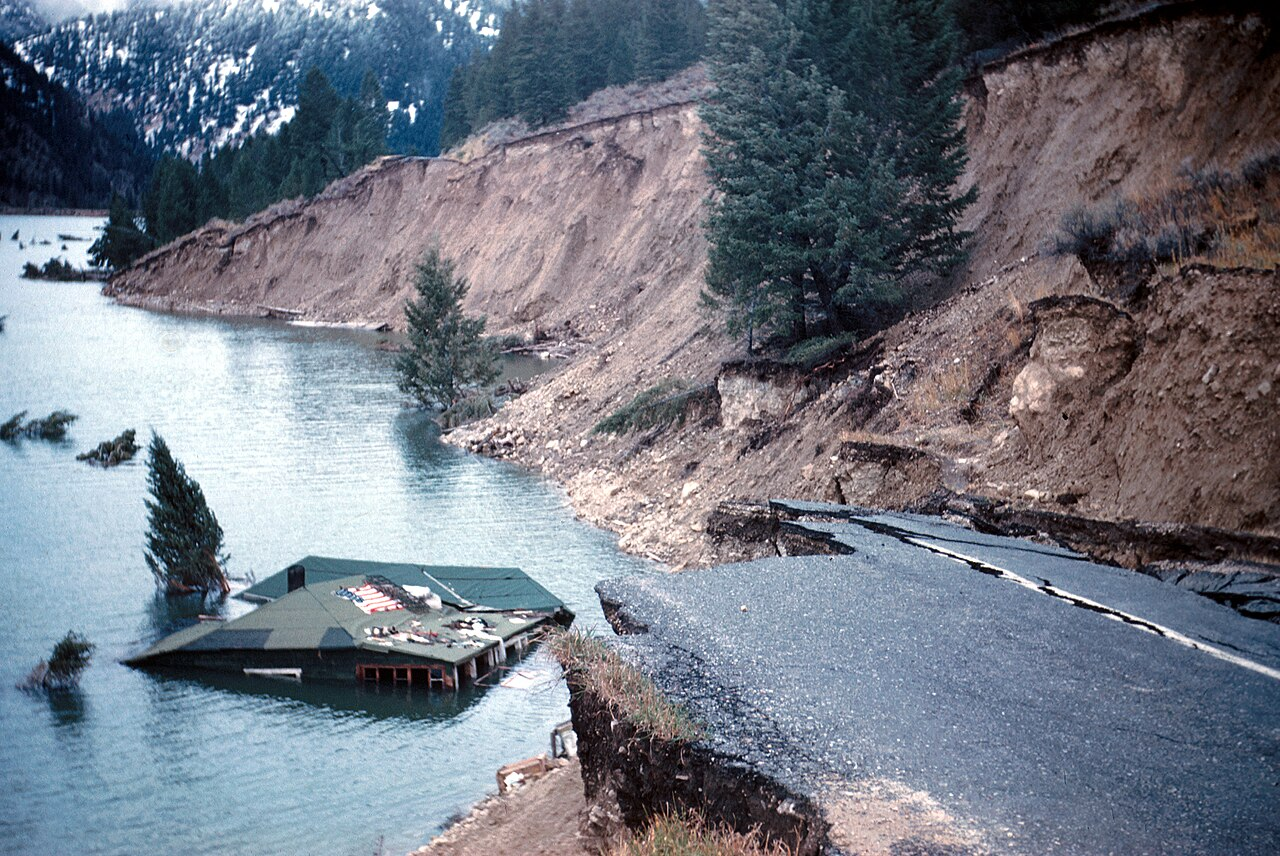
\includegraphics[width=0.6\linewidth]{images/book1/g7-hebgen-road.jpg}

{\small Après le \omterm{def:g4:volcanoes-earthquakes-first-look:earthquake}{séisme} de Hebgen Lake, dans le Montana (États-Unis), en
août 1959~: la route qui longeait le \omterm{def:g1:landscapes-around-us:water}{lac} a glissé dans l'eau, et un
pavillon s'est retrouvé presque sous l'eau. De tels dégâts sont la marque
d'une forte \omterm{def:g7:earthquakes:intensity}{intensité}. Photographie~: I.~J. Witkind, U.S. Geological
Survey (domaine public, via Wikimedia Commons).}
% ledger: commons:hebgen-road, usgs:mmi
\label{fig:g7:earthquakes:hebgen}
\end{omfigure}

\section{Les tsunamis}

\begin{definition}[Tsunami]\label{def:g7:earthquakes:tsunami}
Un \emph{tsunami}\index{tsunami} est une série de vagues marines
déclenchée par un mouvement brusque du fond de la \omterm{def:g2:water-on-earth:ocean}{mer} --- en général un
\omterm{def:g4:volcanoes-earthquakes-first-look:earthquake}{séisme} sous la \omterm{def:g2:water-on-earth:ocean}{mer}, parfois une \omterm{def:g4:volcanoes-earthquakes-first-look:eruption}{éruption} --- qui peut traverser des \omterm{def:g2:water-on-earth:ocean}{océans}
entiers et inonder les \omterm{def:g1:landscapes-around-us:water}{côtes}.
\end{definition}

Quand une \omterm{def:g7:earthquakes:fault}{faille} rompt sous la \omterm{def:g2:water-on-earth:ocean}{mer}, le fond de la \omterm{def:g2:water-on-earth:ocean}{mer} monte ou descend
brusquement, et soulève ou abaisse toute la colonne d'eau qui le surmonte.
L'eau s'étale en vagues. En plein \omterm{def:g2:water-on-earth:ocean}{océan}, un \omterm{def:g7:earthquakes:tsunami}{tsunami} surprend~: il dépasse
rarement un mètre de haut, et les navires ne le remarquent même pas
quand il passe sous eux. Mais il est rapide~: plus de \qty{800}{km/h},
aussi vite qu'un avion de ligne. En arrivant en eau peu profonde, près de
la \omterm{def:g1:landscapes-around-us:water}{côte}, il ralentit jusqu'à 30 ou \qty{50}{km/h} --- encore plus vite que
n'importe quel coureur --- et il grandit. La plupart des \omterm{def:g7:earthquakes:tsunami}{tsunamis} font
moins de \qty{3}{m} de haut à la \omterm{def:g1:landscapes-around-us:water}{côte}~; les plus grands dépassent
\qty{30}{m}. La première vague n'est pas toujours la plus grande, et les
vagues peuvent continuer d'arriver pendant des heures.
% ledger: nws:tsunami-speed, nws:tsunami-safety

\begin{omfigure}
\begin{tikzpicture}[font=\small, x=1cm, y=1cm]
  % sea floor profile: deep ocean on the left, shelf and coast on the right
  \fill[omSea!35] (0,0) -- (13.2,0) -- (13.2,-0.2) -- (11.4,-0.45) -- (10.2,-1.0) -- (8.8,-2.6) -- (0,-2.6) -- cycle;
  \fill[brown!35] (0,-2.6) -- (8.8,-2.6) -- (10.2,-1.0) -- (11.4,-0.45) -- (13.2,-0.2) -- (13.2,0.5) -- (14.2,1.0) -- (14.2,-3.3) -- (0,-3.3) -- cycle;
  % the broken fault under the sea, at left; one block lifted
  \draw[very thick, red!70!black] (1.9,-3.3) -- (2.3,-2.6);
  \draw[-{Stealth[length=2mm]}, thick] (2.75,-3.1) -- (2.75,-2.75);
  \node[anchor=north west, font=\footnotesize, red!70!black] at (0.1,-3.35) {la faille rompt, le fond de la mer fait un saut};
  % wave: low and long in the deep ocean, short and tall near the coast
  \draw[blue!70!black, thick] (0,0) .. controls (1.2,0.18) and (2.2,0.18) .. (3.4,0)
     -- (5.0,0) .. controls (5.8,0.12) and (6.6,0.12) .. (7.4,0) -- (10.6,0)
     .. controls (11.0,0.55) and (11.6,0.9) .. (12.1,0) -- (13.2,0);
  \node[align=center, font=\footnotesize] at (2.0,0.85) {océan profond~: environ 1 m de haut,\\plus de 800 km/h};
  \node[align=center, font=\footnotesize] at (11.1,1.55) {près de la côte~: plus lent\\(30 à 50 km/h), bien plus haut};
  \draw[-{Stealth[length=2.5mm]}, thick, blue!70!black] (4.4,0.45) -- (6.4,0.45);
  \node[font=\footnotesize] at (6.0,-1.5) {des milliers de mètres de profondeur};
  \node[font=\footnotesize] at (12.0,-0.75) {peu profond};
\end{tikzpicture}

{\small Un \omterm{def:g7:earthquakes:tsunami}{tsunami} qui traverse l'\omterm{def:g2:water-on-earth:ocean}{océan} (un dessin, pas à l'échelle~: la
hauteur de la vague est très exagérée). Il est bas et très rapide au-dessus
de l'\omterm{def:g2:water-on-earth:ocean}{océan} profond~; il ralentit et grandit en eau peu profonde, près de la
\omterm{def:g1:landscapes-around-us:water}{côte}.}
% ledger: nws:tsunami-speed
\label{fig:g7:earthquakes:tsunami}
\end{omfigure}

\begin{example}[De Sumatra au Sri Lanka]\label{ex:g7:earthquakes:colombo}
Colombo, la plus grande ville du Sri Lanka, est à environ \qty{1830}{km} de
l'\omterm{def:g7:earthquakes:focus}{épicentre} du \omterm{def:g4:volcanoes-earthquakes-first-look:earthquake}{séisme} de 2004. À \qty{800}{km/h}, un \omterm{def:g7:earthquakes:tsunami}{tsunami} parcourt
cette distance en $1830 \div 800 \approx 2.3$~heures, soit environ
2~heures et 17~minutes. Personne au Sri Lanka n'a senti le \omterm{def:g4:volcanoes-earthquakes-first-look:earthquake}{séisme}~: la
vague est arrivée sans autre avertissement que la \omterm{def:g2:water-on-earth:ocean}{mer} elle-même.
% ledger: nws:tsunami-speed, usgs:largest (distance and time in figdata/grade-7/quake_counts.py, part tsunami)
\end{example}

\begin{remark}[L'avertissement que donne la mer]\label{rem:g7:earthquakes:natural-warning}
% ledger: nws:tsunami-natural-warning, nws:tsunami-speed, shakeout:dch
Sur une \omterm{def:g1:landscapes-around-us:water}{côte}, trois signes peuvent annoncer un \omterm{def:g7:earthquakes:tsunami}{tsunami}~: un \omterm{def:g4:volcanoes-earthquakes-first-look:earthquake}{séisme} fort ou
long~; la \omterm{def:g2:water-on-earth:ocean}{mer} qui se comporte étrangement --- une montée soudaine des eaux,
ou l'eau qui se retire loin du rivage et découvre le fond, comme une marée
très basse~; ou un grondement puissant venu de l'\omterm{def:g2:water-on-earth:ocean}{océan}. Pendant la
secousse, protège-toi comme tu l'as appris (baisse-toi, abrite-toi,
agrippe-toi). Ensuite, n'attends pas d'alerte officielle~: va aussi haut,
ou aussi loin à l'intérieur des terres, que tu le peux, tout de suite. Un
\omterm{def:g7:earthquakes:tsunami}{tsunami} venu d'un \omterm{def:g4:volcanoes-earthquakes-first-look:earthquake}{séisme} proche peut arriver en quelques minutes.
\end{remark}


\section{Exercices}

\begin{exercise}[$\star$]\label{exo:g7:earthquakes:1}
Associe chaque mot à sa définition~: \omterm{def:g7:earthquakes:fault}{faille}~; \omterm{def:g7:earthquakes:focus}{foyer}~; \omterm{def:g7:earthquakes:focus}{épicentre}~;
\omterm{def:g7:earthquakes:seismometer}{sismomètre}~; \omterm{def:g7:earthquakes:magnitude}{magnitude}~; \omterm{def:g7:earthquakes:intensity}{intensité}. (a) L'endroit, en profondeur, où le
glissement commence. (b) La force avec laquelle le sol a tremblé en un
lieu. (c) Une cassure dans les \omterm{def:g3:stones-pebbles-sand:rock}{roches} le long de laquelle les deux côtés se
sont déplacés. (d) Le point de la surface situé au-dessus du \omterm{def:g7:earthquakes:focus}{foyer}. (e) La
taille d'un \omterm{def:g4:volcanoes-earthquakes-first-look:earthquake}{séisme}, un seul nombre par \omterm{def:g4:volcanoes-earthquakes-first-look:earthquake}{séisme}. (f) Un instrument qui
enregistre les secousses du sol.
\end{exercise}

\begin{exercise}[$\star$]\label{exo:g7:earthquakes:2}
Le \omterm{def:g7:earthquakes:focus}{foyer} d'un \omterm{def:g4:volcanoes-earthquakes-first-look:earthquake}{séisme} se trouve \qty{30}{km} juste sous un village.
(a) Où est l'\omterm{def:g7:earthquakes:focus}{épicentre}~? (b) À quelle distance du \omterm{def:g7:earthquakes:focus}{foyer} est le village~?
(c) Un second village est à \qty{40}{km} de l'\omterm{def:g7:earthquakes:focus}{épicentre}. Son \omterm{def:g7:earthquakes:intensity}{intensité}
sera-t-elle en général plus forte ou plus faible que dans le premier
village~? Pourquoi~?
\end{exercise}

\begin{exercise}[$\star$]\label{exo:g7:earthquakes:3}
\omterm{def:g7:earthquakes:magnitude}{Magnitude} ou \omterm{def:g7:earthquakes:intensity}{intensité}~? (a) «~Le \omterm{def:g4:volcanoes-earthquakes-first-look:earthquake}{séisme} a atteint 6.8.~» (b) «~Dans notre
rue, toute la vaisselle est tombée et une cheminée s'est cassée.~» (c)
«~C'était VI en ville et IV dans les villages des \omterm{def:g1:landscapes-around-us:landform}{collines}.~» (d) «~Il a
libéré 32~fois plus d'énergie que celui de l'an dernier.~»
\end{exercise}

\begin{exercise}[$\star$]\label{exo:g7:earthquakes:4}
Vrai ou faux~? Corrige les phrases fausses. (a) Les scientifiques peuvent
dire une semaine à l'avance quand un \omterm{def:g4:volcanoes-earthquakes-first-look:earthquake}{séisme} va frapper. (b) En plein
\omterm{def:g2:water-on-earth:ocean}{océan}, un \omterm{def:g7:earthquakes:tsunami}{tsunami} est un énorme mur d'eau. (c) Un \omterm{def:g4:volcanoes-earthquakes-first-look:earthquake}{séisme} a une seule
\omterm{def:g7:earthquakes:magnitude}{magnitude} mais de nombreuses \omterm{def:g7:earthquakes:intensity}{intensités}. (d) La plupart des grands \omterm{def:g4:volcanoes-earthquakes-first-look:earthquake}{séismes}
se produisent près des \omterm{def:g7:plate-tectonics:plate-boundary}{limites de plaques}.
\end{exercise}

\begin{exercise}[$\star\star$]\label{exo:g7:earthquakes:5}
Utilise le graphique des \omterm{def:g4:volcanoes-earthquakes-first-look:earthquake}{séismes} par an. (a) Environ combien de \omterm{def:g4:volcanoes-earthquakes-first-look:earthquake}{séismes} de
\omterm{def:g7:earthquakes:magnitude}{magnitude} 6 à 6.9 se produisent en un an~? De \omterm{def:g7:earthquakes:magnitude}{magnitude} 7 à 7.9~? (b)
Combien de fois les seconds sont-ils moins nombreux que les premiers~?
(c) Additionne les trois barres à partir de 7~: environ combien de
\omterm{def:g4:volcanoes-earthquakes-first-look:earthquake}{séismes} de \omterm{def:g7:earthquakes:magnitude}{magnitude} 7 ou plus se produisent en un an~? (d) Le graphique
indique 0.04 par an pour une \omterm{def:g7:earthquakes:magnitude}{magnitude} de 9 ou plus. Combien cela
fait-il en 50~ans~?
\end{exercise}

\begin{exercise}[$\star\star$]\label{exo:g7:earthquakes:6}
Utilise la méthode pour comparer des \omterm{def:g7:earthquakes:magnitude}{magnitudes}. (a) Combien de fois plus
d'énergie un \omterm{def:g4:volcanoes-earthquakes-first-look:earthquake}{séisme} de \omterm{def:g7:earthquakes:magnitude}{magnitude} 7 libère-t-il qu'un \omterm{def:g4:volcanoes-earthquakes-first-look:earthquake}{séisme} de \omterm{def:g7:earthquakes:magnitude}{magnitude}
6~? (b) Et un \omterm{def:g4:volcanoes-earthquakes-first-look:earthquake}{séisme} de \omterm{def:g7:earthquakes:magnitude}{magnitude} 8, par rapport à un \omterm{def:g4:volcanoes-earthquakes-first-look:earthquake}{séisme} de \omterm{def:g7:earthquakes:magnitude}{magnitude}
6~? (c) Combien de fois plus grandes sont ses ondes sur le \omterm{def:g7:earthquakes:seismometer}{sismogramme}, à
même distance, entre la \omterm{def:g7:earthquakes:magnitude}{magnitude} 6 et la \omterm{def:g7:earthquakes:magnitude}{magnitude} 8~?
\end{exercise}

\begin{exercise}[$\star\star$]\label{exo:g7:earthquakes:7}
Compte \qty{8}{km} par seconde de décalage entre les ondes rapides et les
ondes lentes. (a) Une station enregistre un décalage de \qty{5}{s}. À
quelle distance était le \omterm{def:g4:volcanoes-earthquakes-first-look:earthquake}{séisme}~? (b) Une autre enregistre \qty{25}{s}.
(c) Un \omterm{def:g4:volcanoes-earthquakes-first-look:earthquake}{séisme} a frappé à \qty{120}{km} d'une station~: quel décalage la
station lira-t-elle~? (d) Pourquoi une seule station ne peut-elle pas dire
où se trouve l'\omterm{def:g7:earthquakes:focus}{épicentre}~?
\end{exercise}

\begin{exercise}[$\star\star$]\label{exo:g7:earthquakes:8}
Utilise le tableau des \omterm{def:g7:earthquakes:intensity}{intensités}. Donne l'\omterm{def:g7:earthquakes:intensity}{intensité} de chaque
témoignage. (a) «~Ressenti par presque tout le monde~; nous avons été
réveillés et deux verres se sont cassés.~» (b) «~Seule ma grand-mère, qui
se reposait à l'étage, l'a senti~; la lampe s'est balancée.~» (c) «~Des
murs et des cheminées sont tombés~; plusieurs maisons se sont effondrées en
partie.~» (d) Le même \omterm{def:g4:volcanoes-earthquakes-first-look:earthquake}{séisme} a donné les témoignages (a) et (c). Explique
comment c'est possible.
\end{exercise}

\begin{exercise}[$\star\star$]\label{exo:g7:earthquakes:9}
Sur les 7\,031 \omterm{def:g4:volcanoes-earthquakes-first-look:earthquake}{séismes} de \omterm{def:g7:earthquakes:magnitude}{magnitude}~6 ou plus de 1976--2025, 5\,561
avaient leur \omterm{def:g7:earthquakes:focus}{foyer} à moins de \qty{70}{km} de profondeur. (a) Combien
avaient un \omterm{def:g7:earthquakes:focus}{foyer} plus profond~? (b) Quel pourcentage cela représente-t-il~?
Arrondis à l'unité. (c) Les \omterm{def:g4:volcanoes-earthquakes-first-look:earthquake}{séismes} profonds se produisent là où une
\omterm{def:g7:plate-tectonics:plate}{plaque} s'enfonce sous une autre. Explique pourquoi ils peuvent y commencer
si profond.
\end{exercise}

\begin{exercise}[$\star\star$]\label{exo:g7:earthquakes:10}
Malé, la capitale des Maldives, est à environ \qty{2500}{km} de
l'\omterm{def:g7:earthquakes:focus}{épicentre} du \omterm{def:g4:volcanoes-earthquakes-first-look:earthquake}{séisme} de 2004. (a) À \qty{800}{km/h}, combien de temps le
\omterm{def:g7:earthquakes:tsunami}{tsunami} a-t-il mis pour l'atteindre~? Donne des heures et des minutes. (b)
Combien de temps après Colombo (2~heures 17~minutes) est-il arrivé~? (c)
Avec de tels délais, pourquoi un système d'alerte aurait-il pu sauver de
nombreuses vies~?
\end{exercise}

\begin{exercise}[$\star\star\star$]\label{exo:g7:earthquakes:11}
Un \omterm{def:g7:earthquakes:tsunami}{tsunami} traverse \qty{400}{km} d'\omterm{def:g2:water-on-earth:ocean}{océan} profond à \qty{800}{km/h}, puis
les \qty{20}{km} d'eau peu profonde de la fin à \qty{40}{km/h}. (a)
Combien de minutes met-il pour la partie profonde~? (b) Pour la partie peu
profonde~? (c) Combien de temps dure tout le trajet~? (d) Qu'y a-t-il de
surprenant dans tes réponses~? (e) Pourquoi la vague grandit-elle en
ralentissant~?
\end{exercise}

\begin{exercise}[$\star\star\star$]\label{exo:g7:earthquakes:12}
(a) Combien de fois plus d'énergie un \omterm{def:g4:volcanoes-earthquakes-first-look:earthquake}{séisme} de \omterm{def:g7:earthquakes:magnitude}{magnitude} 9 libère-t-il
qu'un \omterm{def:g4:volcanoes-earthquakes-first-look:earthquake}{séisme} de \omterm{def:g7:earthquakes:magnitude}{magnitude} 6~? (b) Chaque année, il y a environ
127~\omterm{def:g4:volcanoes-earthquakes-first-look:earthquake}{séismes} de \omterm{def:g7:earthquakes:magnitude}{magnitude} 6 à 6.9. Suppose que chacun libère l'énergie d'un
\omterm{def:g4:volcanoes-earthquakes-first-look:earthquake}{séisme} de \omterm{def:g7:earthquakes:magnitude}{magnitude} 6. Combien d'années de ces \omterm{def:g4:volcanoes-earthquakes-first-look:earthquake}{séismes} faut-il pour libérer
l'énergie d'un seul \omterm{def:g4:volcanoes-earthquakes-first-look:earthquake}{séisme} de \omterm{def:g7:earthquakes:magnitude}{magnitude}~9~? (c) Qu'est-ce que cela
t'apprend sur la part de l'énergie portée par les très grands
\omterm{def:g4:volcanoes-earthquakes-first-look:earthquake}{séismes}~?
\end{exercise}

\section{Problème~: Où le sol a-t-il tremblé~?}

\begin{problem}[{Problème du week-end --- trois stations enregistrent un séisme
sous la mer, l'épicentre est trouvé sur la carte, et la ville de Port
Hale est alertée avant l'arrivée du tsunami}]
\label{pb:g7:earthquakes:1}
% ledger: nws:tsunami-speed, usgs:seismograph, data:prem (figdata/grade-7/epicentre.py)
Un \omterm{def:g4:volcanoes-earthquakes-first-look:earthquake}{séisme} frappe sous la \omterm{def:g2:water-on-earth:ocean}{mer}, le long d'une \omterm{def:g1:landscapes-around-us:water}{côte} inventée. Trois stations
sismiques, A, B et C, se trouvent sur la terre ferme~; la ville de Port
Hale se trouve sur une île (\omterm{def:g2:drawing-to-map:map}{carte} ci-dessous~; un carreau mesure
\qty{20}{km}). Dans cette région, chaque seconde de décalage entre les
ondes rapides et les ondes lentes correspond à \qty{8}{km}. Les stations
enregistrent~:

\begin{center}
\small
\begin{tabular}{|c|c|c|}
\hline
\textbf{station} & \textbf{arrivée des ondes rapides} & \textbf{arrivée des ondes lentes} \\
\hline
A & 10~h~15~min~25~s & 10~h~15~min~45~s \\
B & 10~h~15~min~16~s & 10~h~15~min~29~s \\
C & 10~h~15~min~19~s & 10~h~15~min~34~s \\
\hline
\end{tabular}
\end{center}

\medskip
\noindent\textbf{Partie I --- Trois stations.}\par\nopagebreak
\begin{enumerate}[beginpenalty=10000]
  \item Pour chaque station, trouve le décalage entre les deux arrivées, en
        secondes.
  \item Quelle station est la plus proche du \omterm{def:g4:volcanoes-earthquakes-first-look:earthquake}{séisme}~? Comment le sais-tu
        sans aucun calcul~?
  \item Trouve la distance entre chaque station et le \omterm{def:g4:volcanoes-earthquakes-first-look:earthquake}{séisme}.
  \item La distance de la station A ne dit pas, à elle seule, où était le
        \omterm{def:g4:volcanoes-earthquakes-first-look:earthquake}{séisme}. Décris tous les endroits qui sont à cette distance de A.
\end{enumerate}

\begin{center}
\begin{tikzpicture}
  \begin{axis}[axis equal image, width=12cm, xmin=-60, xmax=360, ymin=-200, ymax=260,
      xtick={-60,-40,...,360}, ytick={-200,-180,...,260}, xticklabels={}, yticklabels={},
      major tick length=0pt,
      axis background/.style={fill=omSea!25}, clip mode=individual]
    \addplot[fill=omLithAlluv, draw=black!50, line width=0.4pt] table[x=x, y=y] {figdata/out/grade-7-epicentre-p-west.dat};
    \addplot[fill=omLithAlluv, draw=black!50, line width=0.4pt] table[x=x, y=y] {figdata/out/grade-7-epicentre-p-north.dat};
    \addplot[fill=omLithAlluv, draw=black!50, line width=0.4pt] table[x=x, y=y] {figdata/out/grade-7-epicentre-p-island.dat};
    % the grid over land and sea, drawn before the labels
    \pgfplotsinvokeforeach{-40,-20,0,20,40,60,80,100,120,140,160,180,200,220,240,260,280,300,320,340}{\draw[black!15] (axis cs:#1,-200) -- (axis cs:#1,260);}
    \pgfplotsinvokeforeach{-180,-160,-140,-120,-100,-80,-60,-40,-20,0,20,40,60,80,100,120,140,160,180,200,220,240}{\draw[black!15] (axis cs:-60,#1) -- (axis cs:360,#1);}
    \addplot[only marks, mark=triangle*, mark size=3.2pt, black,
        nodes near coords, point meta=explicit symbolic,
        nodes near coords style={font=\small\bfseries, anchor=south west}]
      table[x=x, y=y, meta=name] {figdata/out/grade-7-epicentre-p-stations.dat};
    \addplot[only marks, mark=square*, mark size=2.4pt, red!70!black,
        nodes near coords, point meta=explicit symbolic,
        nodes near coords style={font=\small, anchor=north east, fill=omSea!25, inner sep=1pt}]
      table[x=x, y=y, meta=name] {figdata/out/grade-7-epicentre-p-town.dat};
    \draw[-{Stealth[length=2.5mm]}, line width=0.8pt] (axis cs:330,200) -- (axis cs:330,245);
    \node[font=\scriptsize\bfseries, anchor=north] at (axis cs:330,200) {N};
    \node[font=\scriptsize, anchor=west, fill=omLithAlluv, inner sep=1pt] at (axis cs:170,240) {1 carreau = 20 km};
    \fill (axis cs:-60,-200) circle (1.5pt);
    \node[font=\small\bfseries, anchor=north east] at (axis cs:-60,-200) {O};
  \end{axis}
\end{tikzpicture}
\end{center}
% ledger: (invented map: figdata/grade-7/epicentre.py, parts p-west, p-north, p-island, p-stations, p-town)

\medskip
\noindent\textbf{Partie II --- Trouver l'épicentre.}\par\nopagebreak
\begin{enumerate}[resume, beginpenalty=10000]
  \item Un carreau mesure \qty{20}{km}. Combien de carreaux mesure le rayon
        de chaque cercle~?
  \item Place le coin O en bas à gauche de la \omterm{def:g2:drawing-to-map:map}{carte}. La station C est à
        3~carreaux à l'est et 14.5~carreaux au nord de O~; en allant à
        6~carreaux (\qty{120}{km}) plein est depuis C, on arrive en un
        point~E. Vérifie sur la \omterm{def:g2:drawing-to-map:map}{carte} que E est aussi sur les cercles de A
        et de B~: c'est l'\omterm{def:g7:earthquakes:focus}{épicentre}. À combien de carreaux à l'est et au
        nord de O se trouve-t-il~?
  \item L'\omterm{def:g7:earthquakes:focus}{épicentre} est-il sur la terre ferme ou sous la \omterm{def:g2:water-on-earth:ocean}{mer}~? Pourquoi
        est-ce important~?
  \item La \omterm{def:g7:earthquakes:magnitude}{magnitude} était de 7.4. Combien de fois plus d'énergie ce \omterm{def:g4:volcanoes-earthquakes-first-look:earthquake}{séisme}
        a-t-il libérée qu'un \omterm{def:g4:volcanoes-earthquakes-first-look:earthquake}{séisme} de \omterm{def:g7:earthquakes:magnitude}{magnitude}~6.4~?
\end{enumerate}

\medskip
\noindent\textbf{Partie III --- La vague atteint la côte.}\par\nopagebreak
\begin{enumerate}[resume, beginpenalty=10000]
  \item Sur la \omterm{def:g2:drawing-to-map:map}{carte}, Port Hale est à 12~carreaux de l'\omterm{def:g7:earthquakes:focus}{épicentre}. Combien
        de kilomètres cela fait-il~?
  \item À \qty{800}{km/h}, combien de minutes le \omterm{def:g7:earthquakes:tsunami}{tsunami} met-il pour
        atteindre Port Hale~?
  \item Localiser le \omterm{def:g4:volcanoes-earthquakes-first-look:earthquake}{séisme} et envoyer l'alerte prend 5~minutes après le
        début de la secousse. Combien de temps après le \omterm{def:g4:volcanoes-earthquakes-first-look:earthquake}{séisme} l'alerte
        arrive-t-elle à Port Hale~?
  \item Combien de minutes les habitants de Port Hale ont-ils pour gagner
        les hauteurs avant l'arrivée du \omterm{def:g7:earthquakes:tsunami}{tsunami}~?
\end{enumerate}
\end{problem}
